% \documentclass[12pt]{article}
\documentclass[12pt]{ctexart}
\usepackage[utf8]{inputenc}

\usepackage[english]{babel}
\usepackage[dvips]{epsfig}
\usepackage{amsmath}
\usepackage{amssymb}
\usepackage{amsfonts}
\usepackage{amsthm}
\usepackage{amsbsy}
\usepackage{amsgen}
\usepackage{amscd}
\usepackage{amsopn}
\usepackage{amstext}
\usepackage{amsxtra}
\usepackage{mathrsfs}
\usepackage{enumitem}
\usepackage{graphicx}
\usepackage{verbatim}
\usepackage{epstopdf}
\usepackage{float}
\usepackage[all,cmtip]{xy}
\usepackage{accents}
\usepackage{sseq}
\usepackage{url}
\usepackage{hyperref}
\usepackage{makeidx}
\usepackage{siunitx}
\usepackage{xcolor}
\usepackage{physics}

%%%%%%%%% 版面设置 %%%%%%%%%%%%%%%%%%%%%%%%%%%%%%%%%%%%%%
\usepackage{geometry}
\usepackage{titlesec}
\usepackage{fancyhdr}\pagestyle{empty}
\titleformat*{\section}{\large\bfseries}

%
\geometry{
	a4paper,
	total={170mm,240mm},
	left=20mm,
	top=30mm,
}

%Bitte nicht einstellen
\renewcommand{\figurename}{Abbildung}
\renewcommand{\tablename}{Tabelle}
\pagestyle{fancyplain}
\headheight 35pt
\lhead{\name}
\chead{\textbf{\Large \Title}}
\rhead{\due\\\today}
\lfoot{}
\cfoot{}
\rfoot{\small\thepage}
\headsep 1.5em

%%%%%%%%%%%%%%%%%%%%%%%%%%%%%%%%%%%%%%%%%%%%%%%%%%%%%%

\newtheorem{thm}{Theorem}[section]

% 定义解题环境
\theoremstyle{remark}
\newtheorem{remark}[thm]{Remark}
\newtheorem{theorem}{Theorem}
\newtheorem{observation}[thm]{Observation}

\theoremstyle{definition}
\newtheorem{problem}{\text{}}
\newtheorem{Problem}{\text{Problem}}
\newtheorem*{solution}{解}
\newtheorem*{Answer}{Answer}
\newtheorem{example}{Example} 

%%%%%%%%%%%%%%%%%%%%%%%%%%%%%%%%%%%%%%%%%%%%%%%%%%%%%%%%%%%%%%%%%%
\newcommand\name{陈景龙22120307}
\newcommand\due{-}
\newcommand{\emptyline}{\vspace{0.6\baselineskip}}

\newcommand\Title{最优化方法第5次作业}


\begin{document}

\begin{problem}
    用单纯形方法解下列线性规划问题:
    \begin{align*}
        \begin{array}{cl}
            \max & -x_{1}+3 x_{2}+x_{3} \\
            \text { s. t. } & 3 x_{1}-x_{2}+2 x_{3} \leqslant 7 \\
            & -2 x_{1}+4 x_{2} \leqslant 12 \\
            & -4 x_{1}+3 x_{2}+8 x_{3} \leqslant 10 \\
            & x_{1}, x_{2}, x_{3} \geqslant 0 
        \end{array}
    \end{align*}
\end{problem}
\begin{solution}
    引入松弛变量 $x_4, x_5, x_6$,化成标准形式:
    \begin{align*}
        \max& -x_{1}+3 x_{2}+x_{3}\\
        \text { s. t. }& 3 x_{1}-x_{2}+2 x_{3}+x_{4}=7\\
        &-2 x_{1}+4 x_{2}+x_{5}=12 \\
        &-4 x_{1}+3 x_{2}+8 x_{3} \quad+x_{6}=10\\
        &x_{j} \geqslant 0, j=1,2, \cdots, 6 
    \end{align*}
    用单纯形法求解如图\ref{fig1}:
    \begin{figure}[htbp]
        \centering
        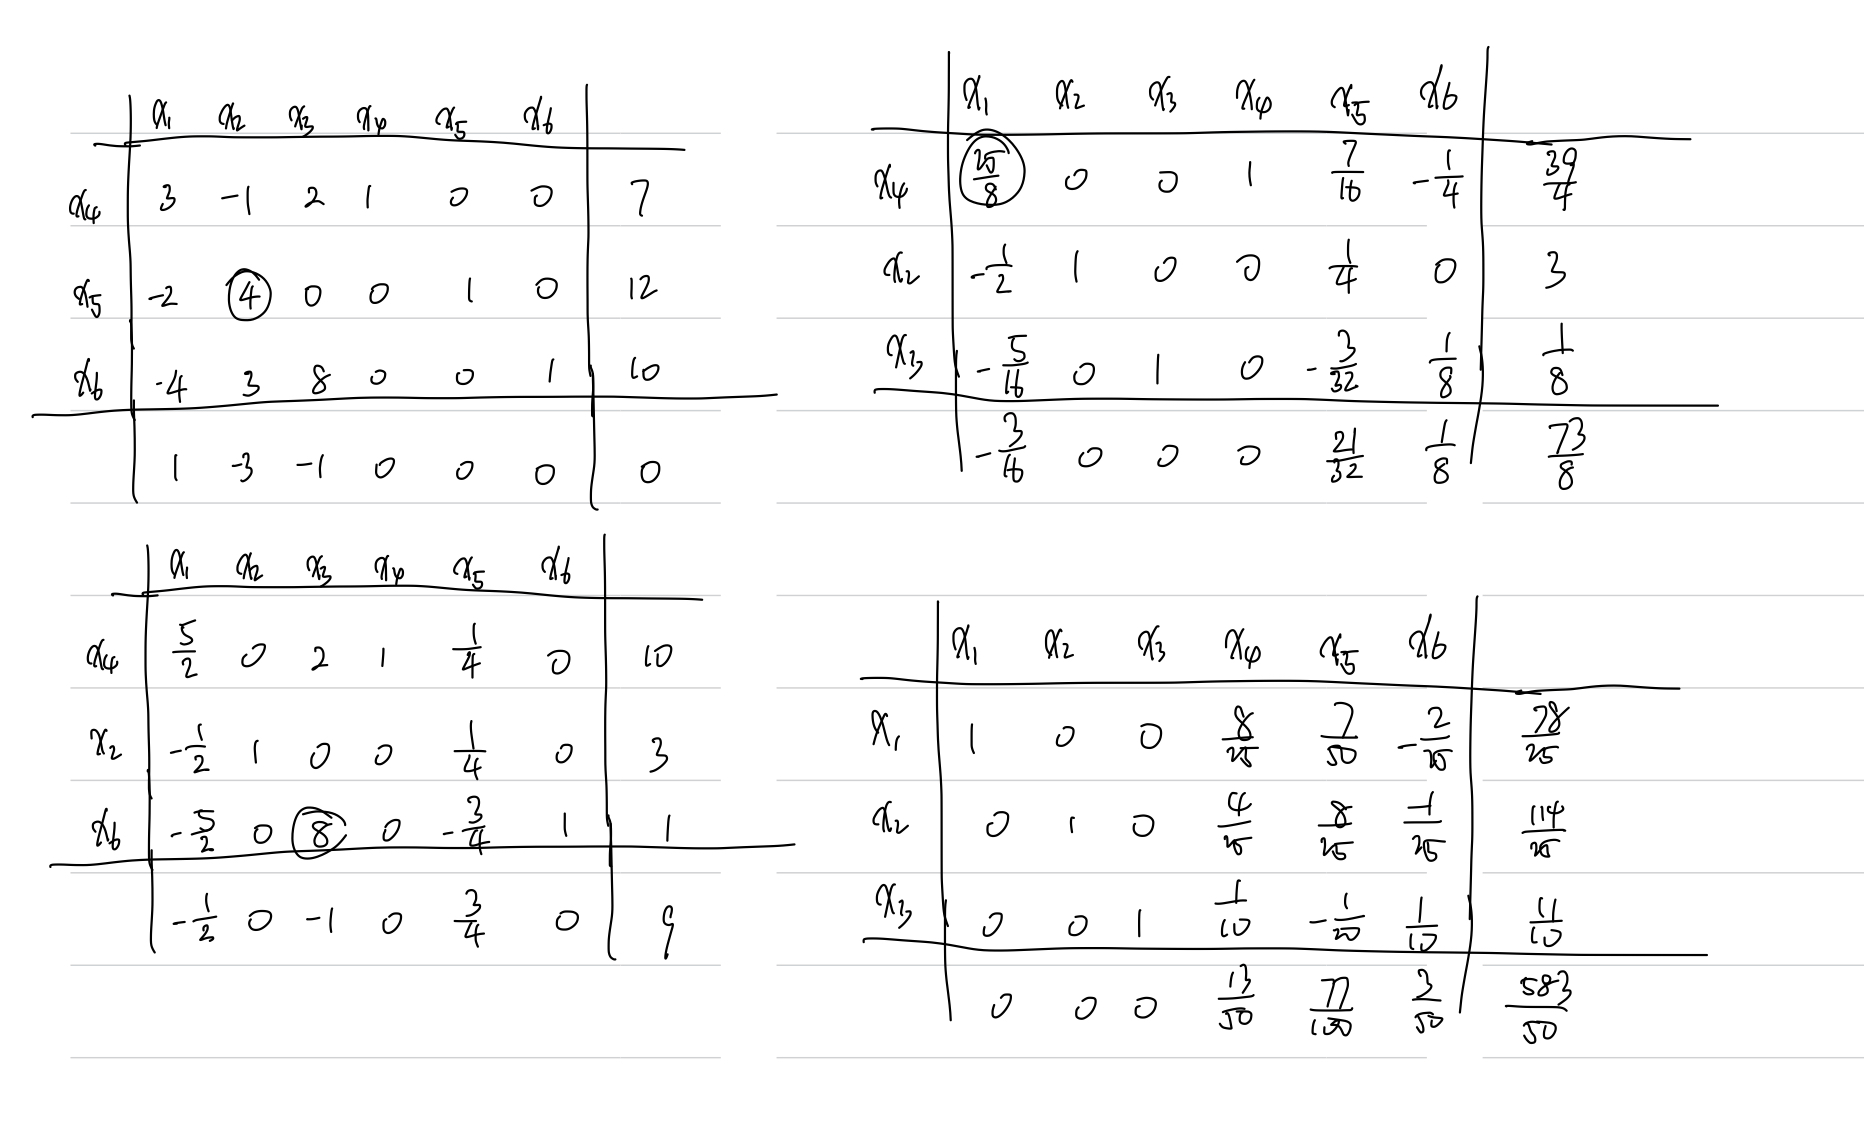
\includegraphics[width=0.8\textwidth]{./figures/img1.png}
        \caption{第一题 \label{fig1}}
    \end{figure}

    最优解 $\bar{x} = \left(\frac{78}{25}, \frac{114}{25}, \frac{11}{10}, 0, 0, 0\right)$,最优值 $f_{max} = \frac{583}{50}$。

\end{solution}

\begin{problem}
    用单纯形方法解下列线性规划问题:
    \begin{align*}
        \begin{array}{ll}
            \min & -3 x_{1}-x_{2} \\
            \text { s. t. } & 3 x_{1}+3 x_{2}+x_{3} \quad=30 \\
            & 4 x_{1}-4 x_{2}+x_{4}=16 \\
            & 2 x_{1}-x_{2} \quad \leqslant 12 \\
            & x_{j} \geqslant 0, \quad j=1, \cdots, 4 
        \end{array}
    \end{align*}
\end{problem}
\begin{solution}
    化成标准形式:
    \[\begin{array}{l}
        \min -3 x_{1}-x_{2}\\
        \text { s. t. } 3 x_{1}+3 x_{2}+x_{3}=30 \text {, }\\
        4 x_{1}-4 x_{2}+x_{4}=16 \text {, }\\
        2 x_{1}-x_{2}+x_{5}=12 \text {, }\\
        x_{j} \geqslant 0, j=1,2, \cdots, 5
    \end{array}\]
    用单纯形法求解如图\ref{fig2}:
    \begin{figure}[htbp]
        \centering
        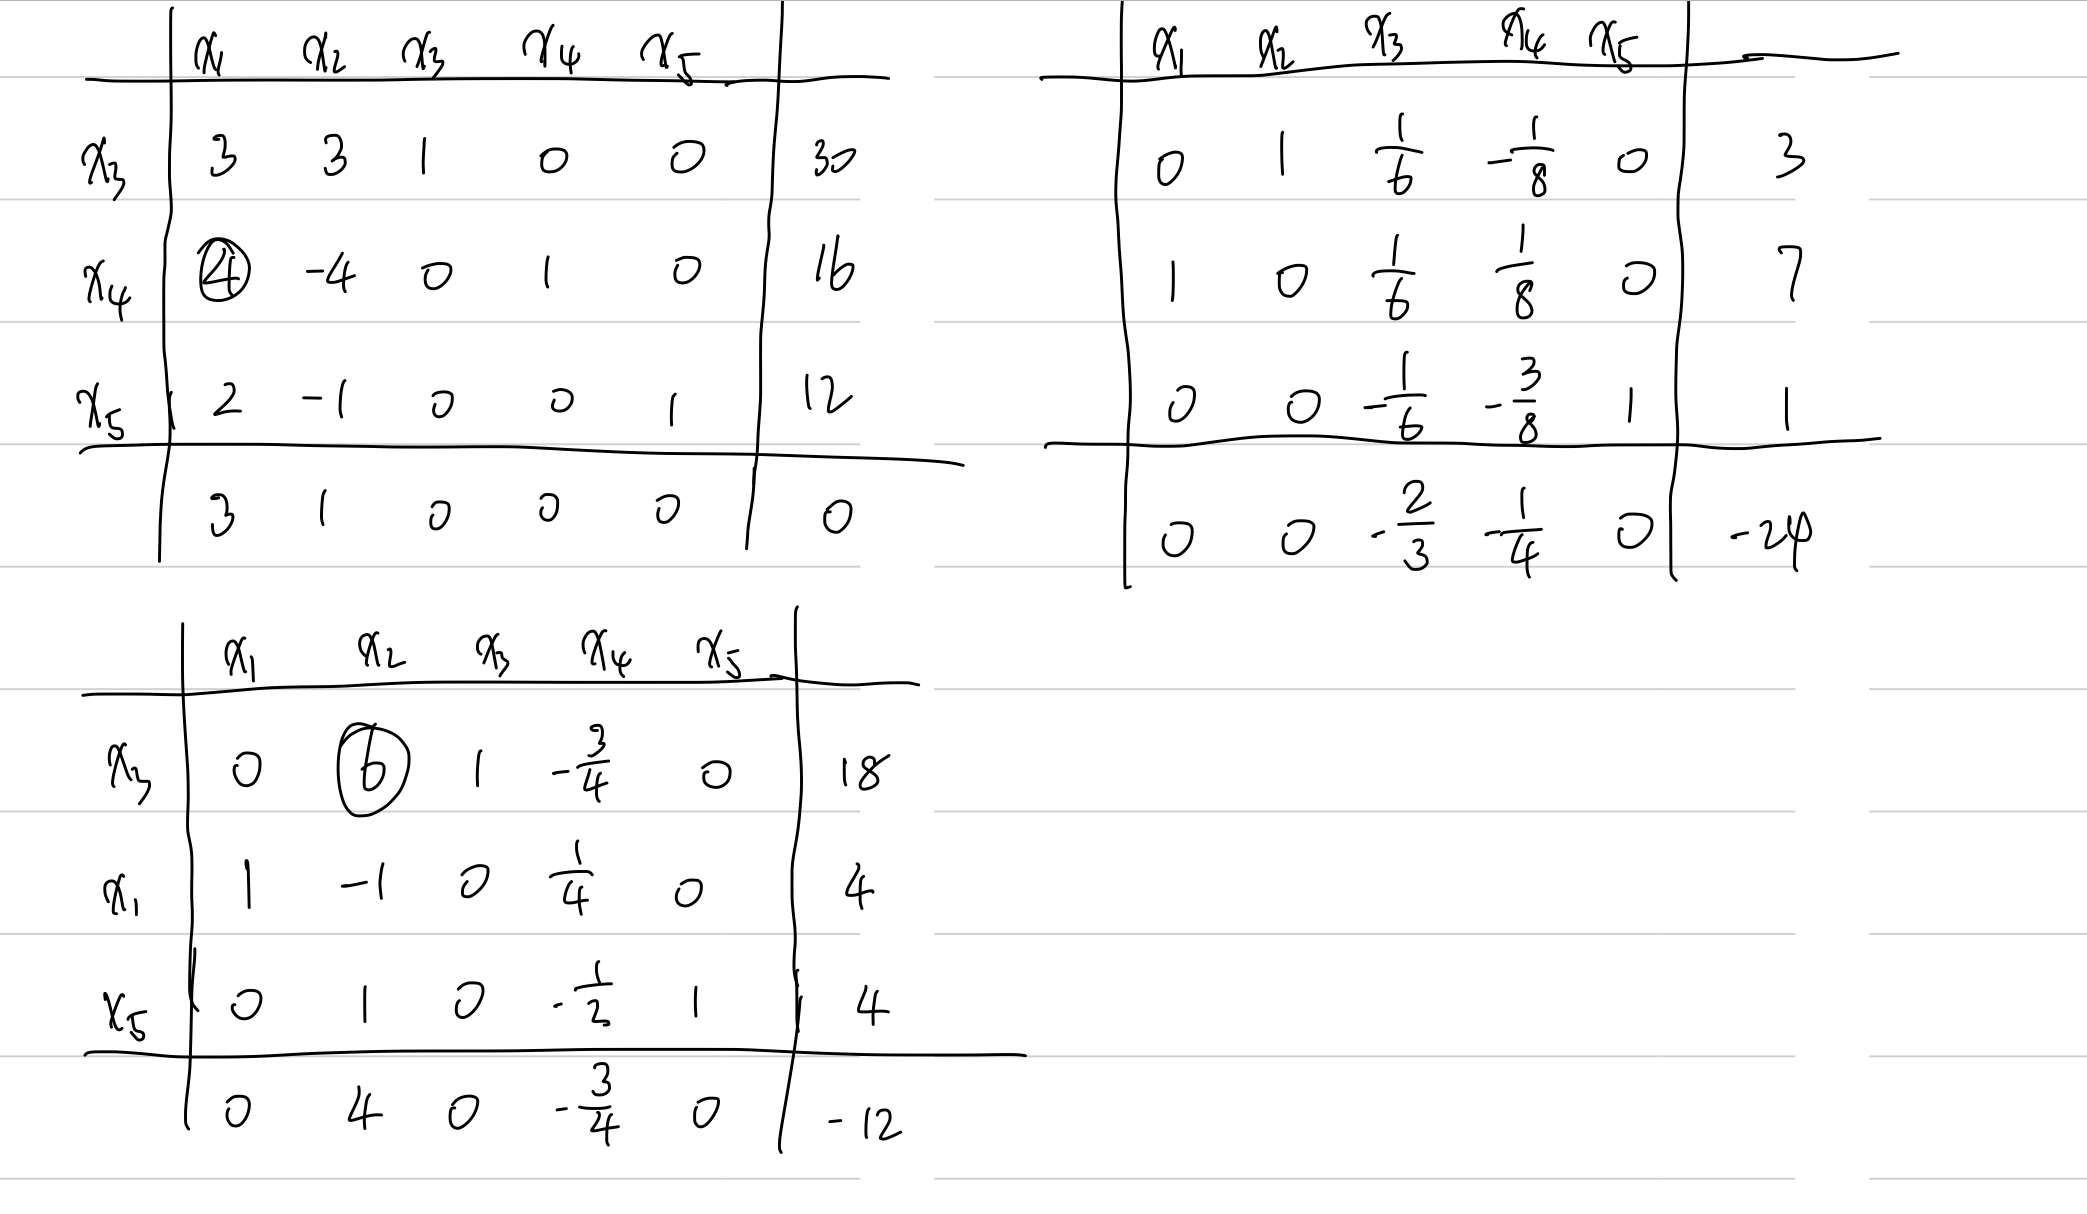
\includegraphics[width=0.8\textwidth]{./figures/img2.png}
        \caption{第二题 \label{fig2}}
    \end{figure}

    最优解 $\bar{x} = (7, 3, 0, 0, 1)$,最优值 $f_{min} = -24$。
\end{solution}

\begin{problem}
    求解下列线性规划问题:
    \[\begin{array}{lc}
        \min & 4 x_{1}+6 x_{2}+18 x_{3} \\
        \text { s. t. } & x_{1}+3 x_{3} \geqslant 3 \\
        & x_{2}+2x_3 \geqslant 5 \\
        & x_{1}, x_{2}, x_{3} \geqslant 0
    \end{array}\]
\end{problem}
\begin{solution}
    化成标准形式:
    \[\begin{array}{ll}
        \min & 4 x_{1}+6 x_{2}+18 x_{3} \\
        \text { s. t. } & x_{1} \quad+3 x_{3}-x_{4}=3, \\
        & x_{2}+2 x_{3}-x_{5}=5, \\
        &x_{j} \geqslant 0, \quad j=1,2, \cdots, 5
    \end{array}\]
    用单纯形法求解如图\ref{fig3}:
    \begin{figure}[htbp]
        \centering
        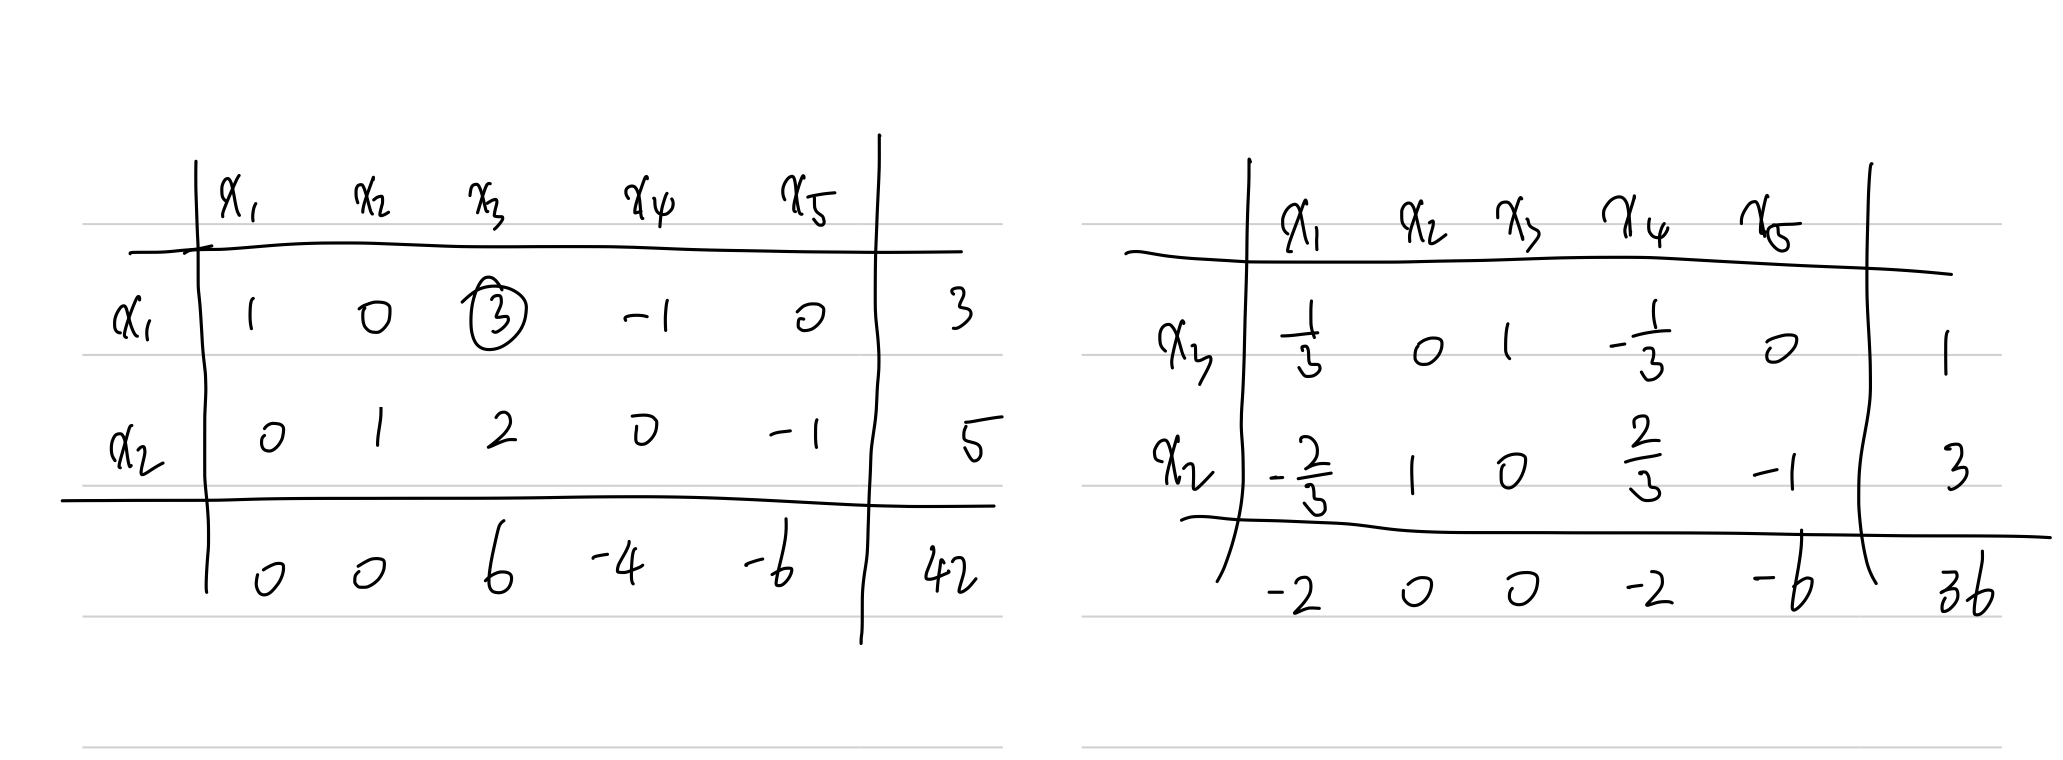
\includegraphics[width=0.8\textwidth]{./figures/img3.png}
        \caption{第三题 \label{fig3}}
    \end{figure}
    最优解 $\bar{x} = (0, 3, 1, 0, 0)$,最优值 $f_{min} = 36$。
    
\end{solution}

\begin{problem}
    求解下列线性规划问题:
    \begin{align*}
        \begin{array}{ll}
            \min & 3 x_{1}-2 x_{2}+x_{3} \\
            \text { s.t. } & 2 x_{1}-3 x_{2}+x_{3}=1 \\
            & 2 x_{1}+3 x_{2} \geqslant 8 \\
            & x_{1}, x_{2}, x_{3} \geqslant 0 
        \end{array}
    \end{align*}
\end{problem}
\begin{solution}
    化成标准形式:
    \begin{align*}
        \min\quad & 3 x_{1}-2 x_{2}+x_{3}  \\
        \text { s. t. } & 2 x_{1}-3 x_{2}+x_{3}  =1 \\
        &2 x_{1}+3 x_{2}  -x_{4}=8, \\
        &x_{j} \geqslant 0, \quad j=1,2,3,4 
    \end{align*}
    引入人工变量 $y$,取大正数 $M$,解下列线性规划:
    \begin{align*}
        \min\quad & 3 x_{1}-2 x_{2}+x_{3}+M y\\
        \text { s.t. }& 2 x_{1}-3 x_{2}+x_{3} =1\\
        &2 x_{1}+3 x_{2}-x_{4}+y=8\\
        &x_{j} \geqslant 0, \quad j=1,2,3,4, \quad y \geqslant 0 
    \end{align*}
    用单纯形法求解如图\ref{fig4}:
    \begin{figure}[htbp]
        \centering
        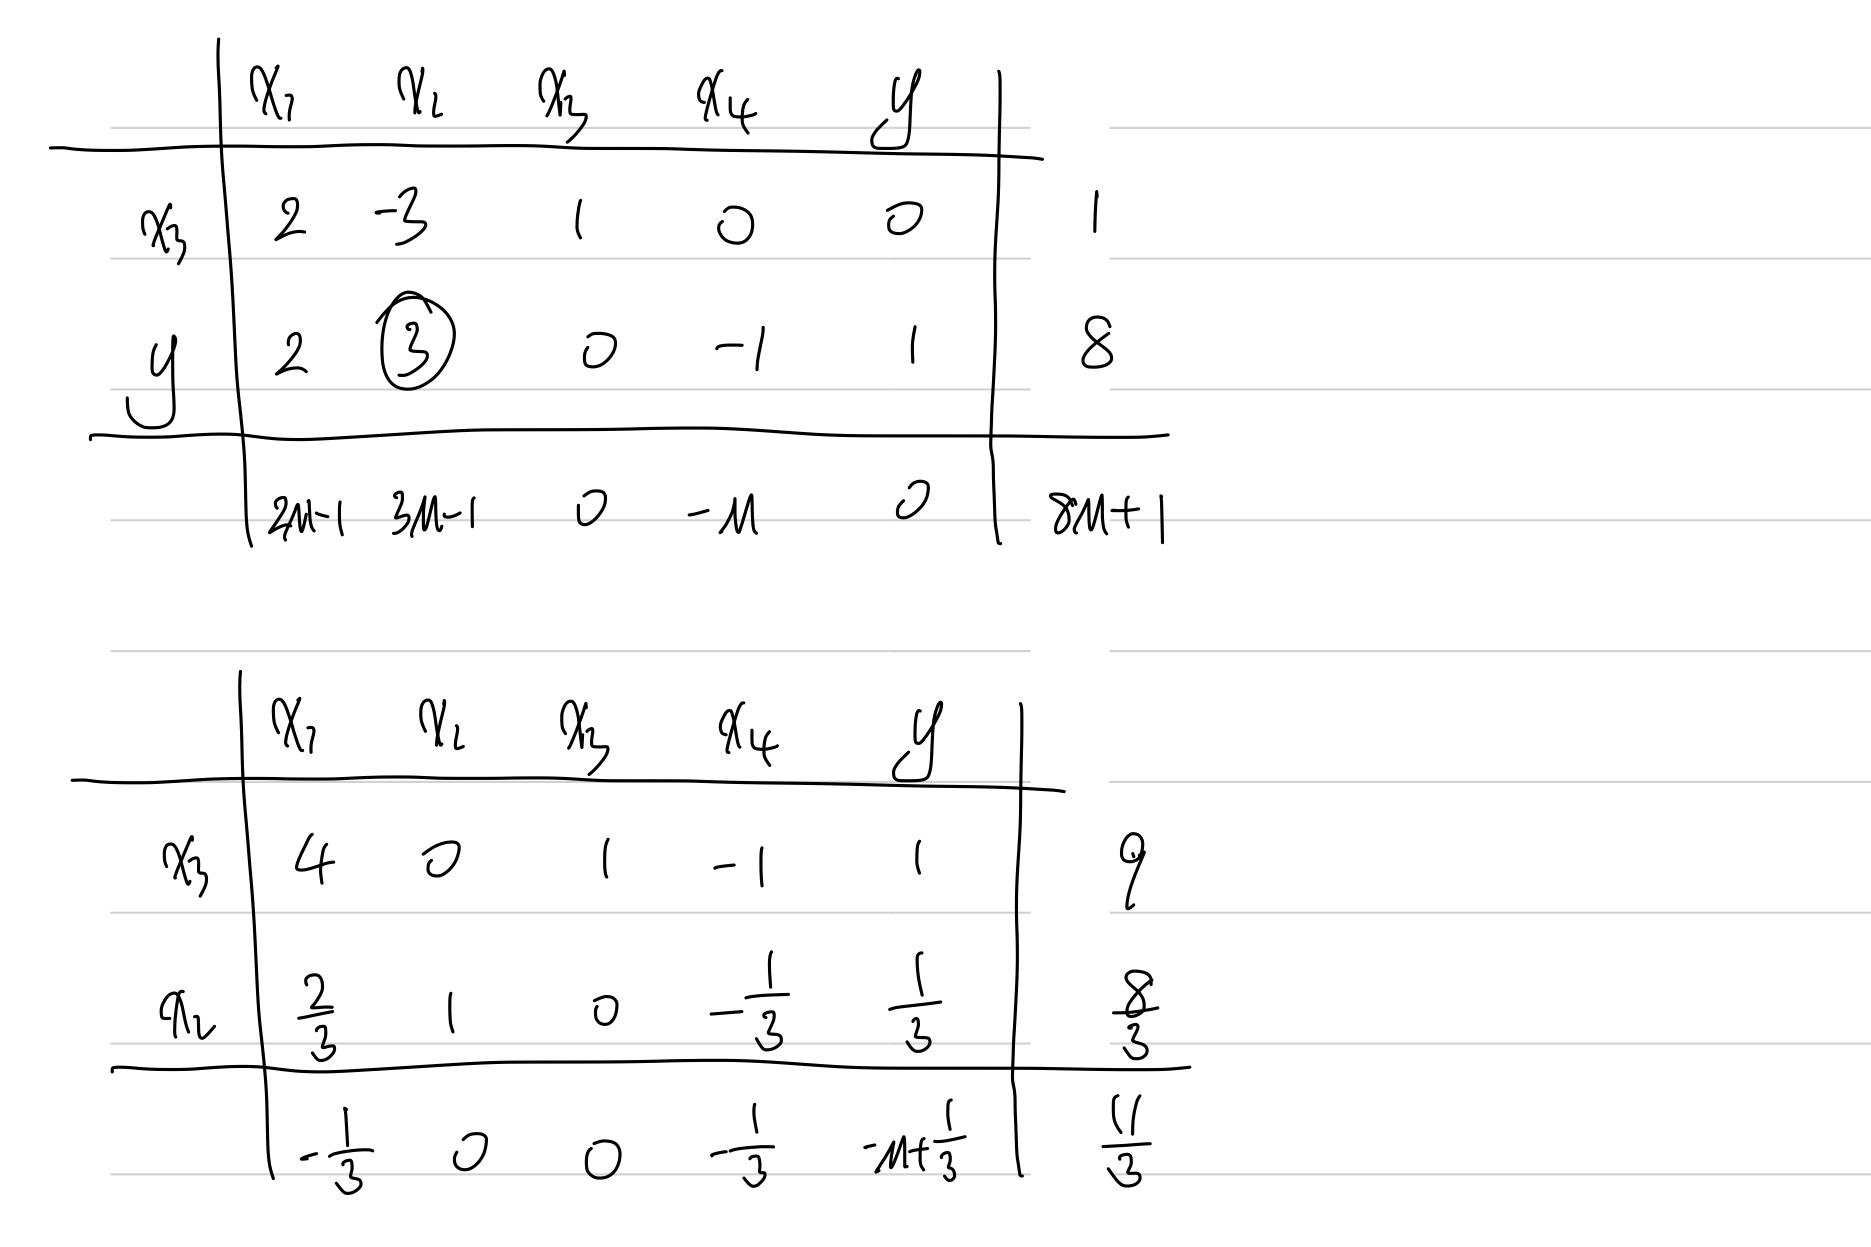
\includegraphics[width=0.8\textwidth]{./figures/img4.png}
        \caption{第四题 \label{fig4}}
    \end{figure}
    最优解 $\bar{x} = \left(0, \frac{8}{3}, 9, 0\right)$,最优值 $f_{min} = \frac{11}{3}$。
\end{solution}

\begin{problem}
    求解下列线性规划问题:
    \begin{align*}
        \begin{array}{l}
            \min 2 x_{1}+x_{2}-x_{3}-x_{4}\\
            \text { s. t. } x_{1}-x_{2}+2 x_{3}-x_{4}=2 \\
            2 x_{1}+x_{2}-3 x_{3}+x_{4}=6 \\
            x_{1}+x_{2}+x_{3}+x_{4}=7 \\
            x_{j} \geqslant 0, \quad j=1, \cdots, 4
        \end{array}
    \end{align*}
\end{problem}
\begin{solution}
    用修正单纯形法求解。初始基本可行解末知,用两阶段法。
    \begin{align*}
        \min \quad& y_{1}+y_{2}+y_{3} \\
        \text { s.t. } \quad &x_{1}-x_{2}+2 x_{3}-x_{4}+y_{1}  =2 \\
        & 2 x_{1}+x_{2}-3 x_{3}+x_{4}+y_{2}  =6\\
        & x_{1}+x_{2}+x_{3}+x_{4}+y_{3}  =7\\
        &x_{j} \geqslant 0, \quad j=1,2,3,4 ; \quad y_{j} \geqslant 0, j=1,2,3 
    \end{align*}
    可得最优解 $\bar{x} = (3, 0, 1, 3)$,最优值 $f_{min} = 2$。
\end{solution}

\begin{problem}
    假设用单纯形方法解线性规划问题。
    \begin{align*}
        \begin{array}{ll}
            \min & \boldsymbol{c x} \\
            \text { s. t. } & \boldsymbol{A x}=\boldsymbol{b}, \\
            & \boldsymbol{x} \geqslant \mathbf{0 .} .
        \end{array}
    \end{align*}
    在某次迭代中对应变量 $x_j$ 的判别数 $z_j - c_j > 0$,且单纯性表中相应的列 $y_i = B^{-1}p_j \le 0$,证明 \[d = \begin{bmatrix}
        -y_i\\
        0\\
        \vdots\\
        1\\
        \vdots\\
        0
    \end{bmatrix}\]
    是可行域的极方向,其中分量 $1$ 对应 $x_j$。
\end{problem}
\begin{solution}
    记 \[A = \begin{bmatrix}
        p_1 & \cdots & p_m & \cdots & p_n
    \end{bmatrix} = \begin{bmatrix}
        B & p_{m + 1} & \cdots & p_n
    \end{bmatrix}\]
    由于\[Ad = \begin{bmatrix}
        B & p_{m + 1} & \cdots & p_j & \cdots & p_n
    \end{bmatrix}\begin{bmatrix}
        -B^{-1}p_j \\
        0\\
        \vdots\\
        1\\
        \vdots\\
        0
    \end{bmatrix} = -p_j + p_j = 0\]
    且 $d\geqslant 0$,因此 $d$ 是可行域的方向。
    
    设 $d$ 可表示成可行域的两个方向 $d^{(1)}$ 和 $d^{(2)}$ 的正线性组合,即 $d = \lambda d^{(1)} + \mu d^{(2)}$,则
    \[\boldsymbol{d}^{(1)}=\left[\begin{array}{c}
        \boldsymbol{d}_{\mathbf{B}}^{(1)} \\
        0 \\
        \vdots \\
        a_{j} \\
        \vdots \\
        0
        \end{array}\right], \quad \boldsymbol{d}^{(2)}=\left[\begin{array}{c}
        \boldsymbol{d}_{\mathbf{B}}^{(2)} \\
        0 \\
        \vdots \\
        b_{j} \\
        \vdots \\
        0
    \end{array}\right], \quad a_{j}, b_{j}>0\]
    由于 $d^{(1)}$ 是可行域方向,因此 $Ad^{(1)} = 0, d^{(1)}\geqslant 0$,即 $Bd_B^{(1)} + a_jp_j = 0$,同理 $Bd_B^{(2)} + b_jp_j = 0$,可以得到 $\frac{1}{a_{j}} \boldsymbol{B} \boldsymbol{d}_{\boldsymbol{B}}^{(1)}=\frac{1}{b_{j}} \boldsymbol{B} \boldsymbol{d}_{\boldsymbol{B}}^{(2)}$,即 $\boldsymbol{d}_{\mathbf{B}}^{(2)}=\frac{b_{j}}{a_{j}} \boldsymbol{d}_{\mathbf{B}}^{(1)}$。代入方向 $d^{(2)}$,得到 $\boldsymbol{d}^{(2)}=\frac{b_{j}}{a_{j}} \boldsymbol{d}^{(1)}$。即 $d^{(1)},d^{(2)}$ 是同向非零向量,因此方向 $d$ 不能表示成两个不同方向的正线性组合,因此 $d$ 是可行域的方向。
\end{solution}

\end{document}